\chapter{GeoPaxos with b+tree}\label{sec:geopaxos-with-b+tree}
Now that we have discussed the needed background, we can move onto the next step: using a b+tree on top of GeoPaxos to store the data objects. A b+tree has many interesting characteristics that make it particularly suitable for some types of applications, but it also brings some new challenges to the table. The data structure has to be indentically replicated in every replica: this means that all the operations done on the tree have to be deterministic and executed in the right order. While this is not particularly complicated on other data structures, such as a HashMap, this becomes more complicated with a tree, where we have many branches and nodes that may split and change the whole structure of the tree.

Furthermore, the usage of GeoPaxos and a tree brings the need for a new type of operation. In GeoPaxos the objects are assigned to one or more groups, depending on the type, number and origin of accesses. Of these groups, one will also be chosen in each replica to be the preferred partition for the operation, usually based on geographic location. There has to be a moment when these groups are decided and calculated for each object in the b+tree. For this, we have a command called repartition. The command takes the workload of an object, which is the number of reads and writes from each group on this object, and a graph that represents the geographic location of the various replicas. It then calculates the optimal placement of the object in the groups, that with the given workload would give us the minimum average latency. This operation can take be a big performance bottleneck, since it has to be executed for every object in the tree, and since we have to consider every combination of groups it scales exponentially on the number of groups. We therefore want to find a fast way to perform this operation so that we still get the right assignment of objects in a short amount of time.

In this chapter I will first explain what a b+ tree is, how it works and what are its advantages and disadvantages. I will then describe the specific b+ tree used in our application. Then I will go over the various approaches that were attempted to improve the performance of the repartition optimization, followed with tests on the performance of the repartition only and finally with GeoPaxos as well.

\section{B+ tree}\label{sec:B+tree}
[maybe say first what a b-tree is]

A B+ tree is an N-ary tree with a variable but often large number of children per node. A B+ tree consists of a root, internal nodes and leaves.[1] The root may be either a leaf or a node with two or more children.[2]

A B+ tree can be viewed as a B-tree in which each node contains only keys (not key–value pairs), and to which an additional level is added at the bottom with linked leaves.

The primary value of a B+ tree is in storing data for efficient retrieval in a block-oriented storage context — in particular, filesystems. This is primarily because unlike binary search trees, B+ trees have very high fanout (number of pointers to child nodes in a node,[1] typically on the order of 100 or more), which reduces the number of I/O operations required to find an element in the tree.

The order, or branching factor, b of a B+ tree measures the capacity of nodes (i.e., the number of children nodes) for internal nodes in the tree. The actual number of children for a node, referred to here as m, is constrained for internal nodes so that $\lceil b/2\rceil \leq m\leq b$. The root is an exception: it is allowed to have as few as two children.[1] For example, if the order of a B+ tree is 7, each internal node (except for the root) may have between 4 and 7 children; the root may have between 2 and 7. Leaf nodes have no children, but are constrained so that the number of keys must be at least $\lceil b/2 \rceil$  and at most b. In the situation where a B+ tree is nearly empty, it only contains one node, which is a leaf node. (The root is also the single leaf, in this case.) This node is permitted to have as little as one key if necessary and at most b-1.

\begin{figure}[htb]
    \centering
    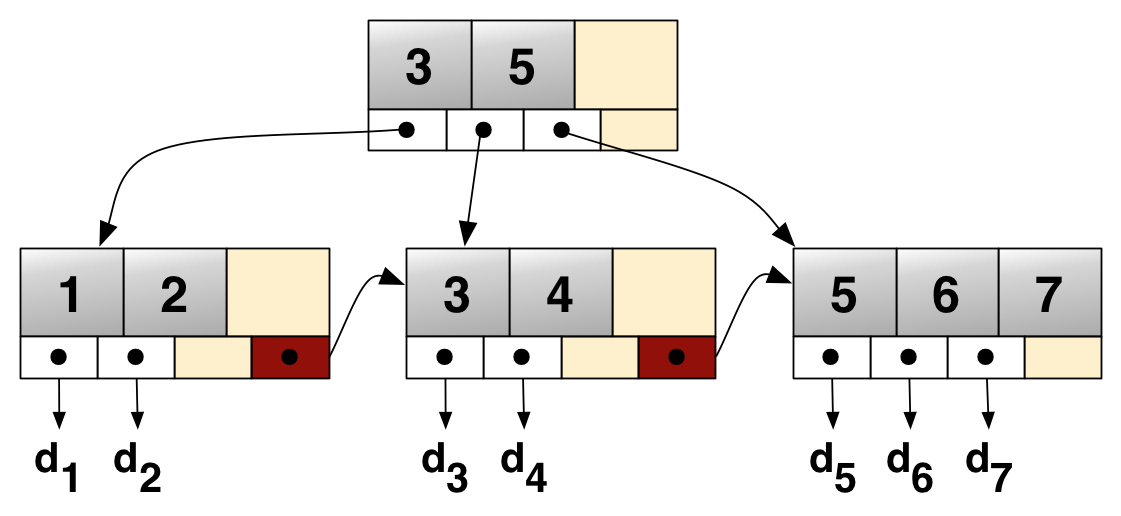
\includegraphics{img/b+tree.png}
    \caption[The architecture of the system]{ The architecture of the system. The
      \textit{Viper IDE} and \textit{Viper Debugger} boxes denote, respectively,
      the main Viper extension and the new debugger extension. They both interact,
      independently, with Visual Studio Code. Viper Server is responsible for
      running the verification backends.}
    \label{fig:b+tree}
\end{figure}

[add characteristics from wiki]

Insertion[edit]
Perform a search to determine what bucket the new record should go into.
If the bucket is not full (at most b-1 entries after the insertion), add the record.
Otherwise, before inserting the new record
split the bucket.
original node has $\lceil(L+1)/2\rceil$ items
new node has $\lfloor(L+1)/2\rfloor$ items
Move $\lceil(L+1)/2\rceil$-th key to the parent, and insert the new node to the parent.
Repeat until a parent is found that need not split.
If the root splits, treat it as if it has an empty parent and split as outline above.
B-trees grow at the root and not at the leaves.[1]


[explain the statistics, how/when they're upadted, node splitting, aging]
\section{Optimization approaches}\label{sec:optimization-approaches}

\subsection{group by level(bucket)}\label{sec:fixed-size buckets}
[pic of grouped levels]

\subsection{dynamic bucket}\label{sec:variable-size buckets}
if few reads compared to parent, inherit
[pic of grouped levels]

\subsection{hot groups}\label{sec:hot-groups}

\subsection{LRU caching}\label{sec:LRU caching}

\section{Optimization tests}\label{sec:optimization-tests}

\section{GeoPaxos tests}\label{sec:geopaxos-tests}
[say how the clients act, put a skew graph, different types of clients, repartitino timings...]